%  Add 'draft' option to mark overfull boxes with black boxes
%  Add 'showkeys' option to make keywords appear
\documentclass[
aps,
reprint,
amsmath, amssymb,
%preprint,
superscriptaddress,
%groupedaddress
]{revtex4-2}
\usepackage[spanish]{babel}
\usepackage{float}
\usepackage{graphicx}
\usepackage{dcolumn}
\usepackage{bm}
\usepackage{physics}
\renewcommand{\andname}{y}
\renewcommand{\spanishtablename}{Tabla}
\begin{document}
\preprint{Universidad de Córdoba}
% Use the \preprint command to place your local institutional report number in the upper righthand corner of the title page in preprint mode.
%\preprint{}

%Title of paper
\title{Análisis de las propiedades \\de la Reflexión y Refracción de luz}

\author{Luis Miguel Patiño Buendía}
\author{Jesús Manuel Gallego Mercado}

\affiliation{Universidad de Córdoba.\\ Montería-Córdoba, Colombia}

%\email[]{Your e-mail address}
%\homepage[]{Your web page}
%\thanks{}


\date{\today}

\begin{abstract}
En el siguiente informe de laboratorio se estudió el comportamiento de un haz de luz que incide desde medios de alto índice refractivo hacia medios de menor índice refractivo y viceversa; asimismo, se intentó corroborar el valor del índice de refracción del agua y se estudió lo que ocurre cuando la luz incide sobre un recipiente transparente con agua al cual se introduce un lápiz. Todo esto con el objetivo de estudiar las propiedades de la reflexión y la refracción de la luz que se derivan de la ley de Snell. Para esto, se hizo incidir mediante un foco de luz, un haz sobre un recipiente con agua que tenía forma cilíndrica y semicircular y que estaba ubicado sobre un disco de Hartl. Esto también se hizo con un cilindro de vidrio. Por otra parte, se introdujo agua y un lapiz en un vaso de precipitados y se realizaron fotografías en diferentes ángulos. Se concluyó que bajo la condición de que el índice de refracción de los medios $n_i  > n_t$, para cierto ángulo límite o ángulo crítico, el haz de luz refractado desaparece y por ende, toda la luz es reflejeda. La razón de este fenómeno se asocia a que la alta densidad de los medios reduce la velocidad de propagación del haz de luz.
\end{abstract}


%\keywords{}
\maketitle
% References should be done using the \cite, \ref, and \label commands
\section{Introducción}
El estudio sistemático de los fenómenos que experimenta la materia y su interacción diaria con el hombre, lo han llevado a la necesidad de entender de manera profunda y específica la manera en como estos funcionan, a fin de predecir el comportamiento del espacio en que habita. El propósito de esta práctica, radica en el estudio de la luz como onda electromagnética en el campo de la óptica geométrica. Más específicamente, estudiar las propiedades de \textit{reflexión y refracción} de un rayo de luz que incide con carcteristicas especificas y ``controladas'' a la hora de realizar el experimento.

\section{Reflexión y Refracción}
La reflexión y la refracción de la luz son dos fenómenos físicos que puede experimentar un rayo de luz. En la reflexión, el rayo de luz rebota sobre una superficie, mientras en la refracción el rayo de luz que pasa de un medio a otro cambia su ángulo de propagación.

\subsection{Reflexión de la Luz}

En la reflexión de la luz se puede distinguir el rayo original o rayo incidente y el rayo que se devuelve o rayo reflejado. En el punto donde el rayo incidente y el reflejado se encuentran, se traza una línea imaginaria perpendicular a la superficie que se conoce como normal.\\
\\
Entre el rayo incidente y la normal se forma el ángulo de incidencia, y entre la normal y el rayo reflejado se forma el ángulo de reflexión. Estos ángulos son iguales \cite{optics}.\\
\\
\subsection{Reflexión Interna Total}

Este fenómeno sólo se produce para ángulos de incidencia superiores a un cierto valor límite o crítico $\theta_c$ donde el rayo de luz refractado no es capaz de atravesar la superficie entre ambos medios y por ende se refleja completamente. La reflexión interna total solamente ocurre en rayos que viajan de un medio de alto índice refractivo hacia medios de menor índice de refracción. El ángulo límite o crítico viene dado por: 

\begin{align*}
    \theta_{c} = \sin^{-1}\left(\frac{n_{2}}{n_{1}}\right)
\end{align*}


\subsection{Refracción de la Luz}

La refracción de la luz se produce en la superficie de separación de los medios de diferente densidad;lo que afecta la velocidad de propagación de la luz. El desvío de la dirección de propagación será mayor a mayor diferencia de la velocidad de propagación en los dos medios.\\
\\
En la refracción de la luz se distingue el rayo incidente y el rayo refractado. Entre el rayo incidente y la línea normal se forma el ángulo de incidencia $\theta_i$. Mientras que entre el rayo refractado y la normal se forma el ángulo de refracción $\theta_t$ \cite{optics}.\\


\textbf{Leyes de la Refracción de la Luz}

\begin{itemize}
    \item Los índices de refracción $n_1$ y $n_2$, el ángulo de incidencia $\theta_{i}$ y el ángulo del haz refractado o transmitido $\theta_{t}$ se relacionan por la siguiente expresión:
    
    \begin{equation}
        \label{eqn:ley_snell}
        n_{1} \sin{\theta_{i}} = n_{2} \sin{\theta_{t}} 
    \end{equation}
\end{itemize}

\textbf{Índice de refracción}\\
\\
Se denomina índice de refracción al cociente de la velocidad de la luz en el vacío y la velocidad de la luz en el medio cuyo índice se calcula. Se simboliza con la letra $n$ y se trata de un valor adimensional.

\begin{align}
    n = \dfrac{c}{v}
\end{align}

Donde
\begin{itemize}
    \item $c =$ Velocidad de la luz en le vacío
    \item $v =$ Velocidad de la luz en el medio cuyo índice se calcula (agua, vidrio, etc.)
\end{itemize}


\section{Objetivos}
\begin{enumerate}
    \item Estudiar las propiedades de la refracción y reflexión de la luz derivadas de la ley de Snell.
    \begin{itemize}
        \item Determinar el ángulo en el cual un haz de luz posee reflexión interna total y bajo qué condiciones ocurre.
        \item Estimar el índice de refracción del agua.
        \item Analizar cualitativamente lo que ocurre con la luz que incide sobre un recipiente con agua y un lápiz dentro de éste.
    \end{itemize}
\end{enumerate}

\section{\label{sec:expe}Experimento y Metodología}
\begin{table}[H]
	\caption{\label{tab:materiales}Materiales e Instrumentos de medida.}
	\begin{ruledtabular}
		\begin{tabular}{lcc}
            \textrm{Materiales} & \textrm{Referencia} & \textrm{Cantidad}\\
			\colrule
            Banco Óptico                & --------- & 1\\
			Diafragma con una Ranura    & --------- & 1\\
            Disco de Hartl              & --------- & 1\\
            Foco Luminoso               & --------- & 1\\
            Lente de $f'=+50mm, 40\Phi$ & --------- & 1\\
            Sección de lente semicircular & --------- & 1\\
            $R=+25mm$      & &\\
            Soporte para foco y disco   & --------- & 2\\
            Soporte para diafragma      & --------- & 1\\
            Espejo                      & --------- & 1\\
            Transformador S. $12V-20W$  & --------- & 1\\
            Vaso de Precipitados & --------- & 1\\
            Lápiz & --------- & 1\\
	\end{tabular}
	\end{ruledtabular}
\end{table}

El experimento se dividió en 3 partes:
\begin{enumerate}
    \item Se hizo incidir un haz de luz sobre el centro de la cara plana de un cilindro semicircular lleno de agua que se encontraba sobre un disco de Hartl. Al girar el disco se tomaron medidas del ángulo de incidencia, refracción y reflexión. El montaje es expuesto en la figura \ref{fig:img_1}.
    
    \item Posteriormente, y mediante el mismo montaje, se hizo incidir el haz de luz sobre el centro de la cara curva del cilindro semicircular lleno de agua (se realizó también con un cilindro de vidrio) se anotaron los ángulos de inicidencia, reflexión y refracción. Para un cierto ángulo de incidencia el haz refractado desaparece, este ángulo está consignado en los resultados.
    
    \item En un vaso de precipitados casi transparente se llenó con cierto volúmen de agua y se introdujo un lápiz dentro del vaso. Mediante una cámara digital, se tomaron fotografías en diferentes ángulos: frontal, trasero y lateral. 
    
    
\end{enumerate}

\begin{figure}
\centering
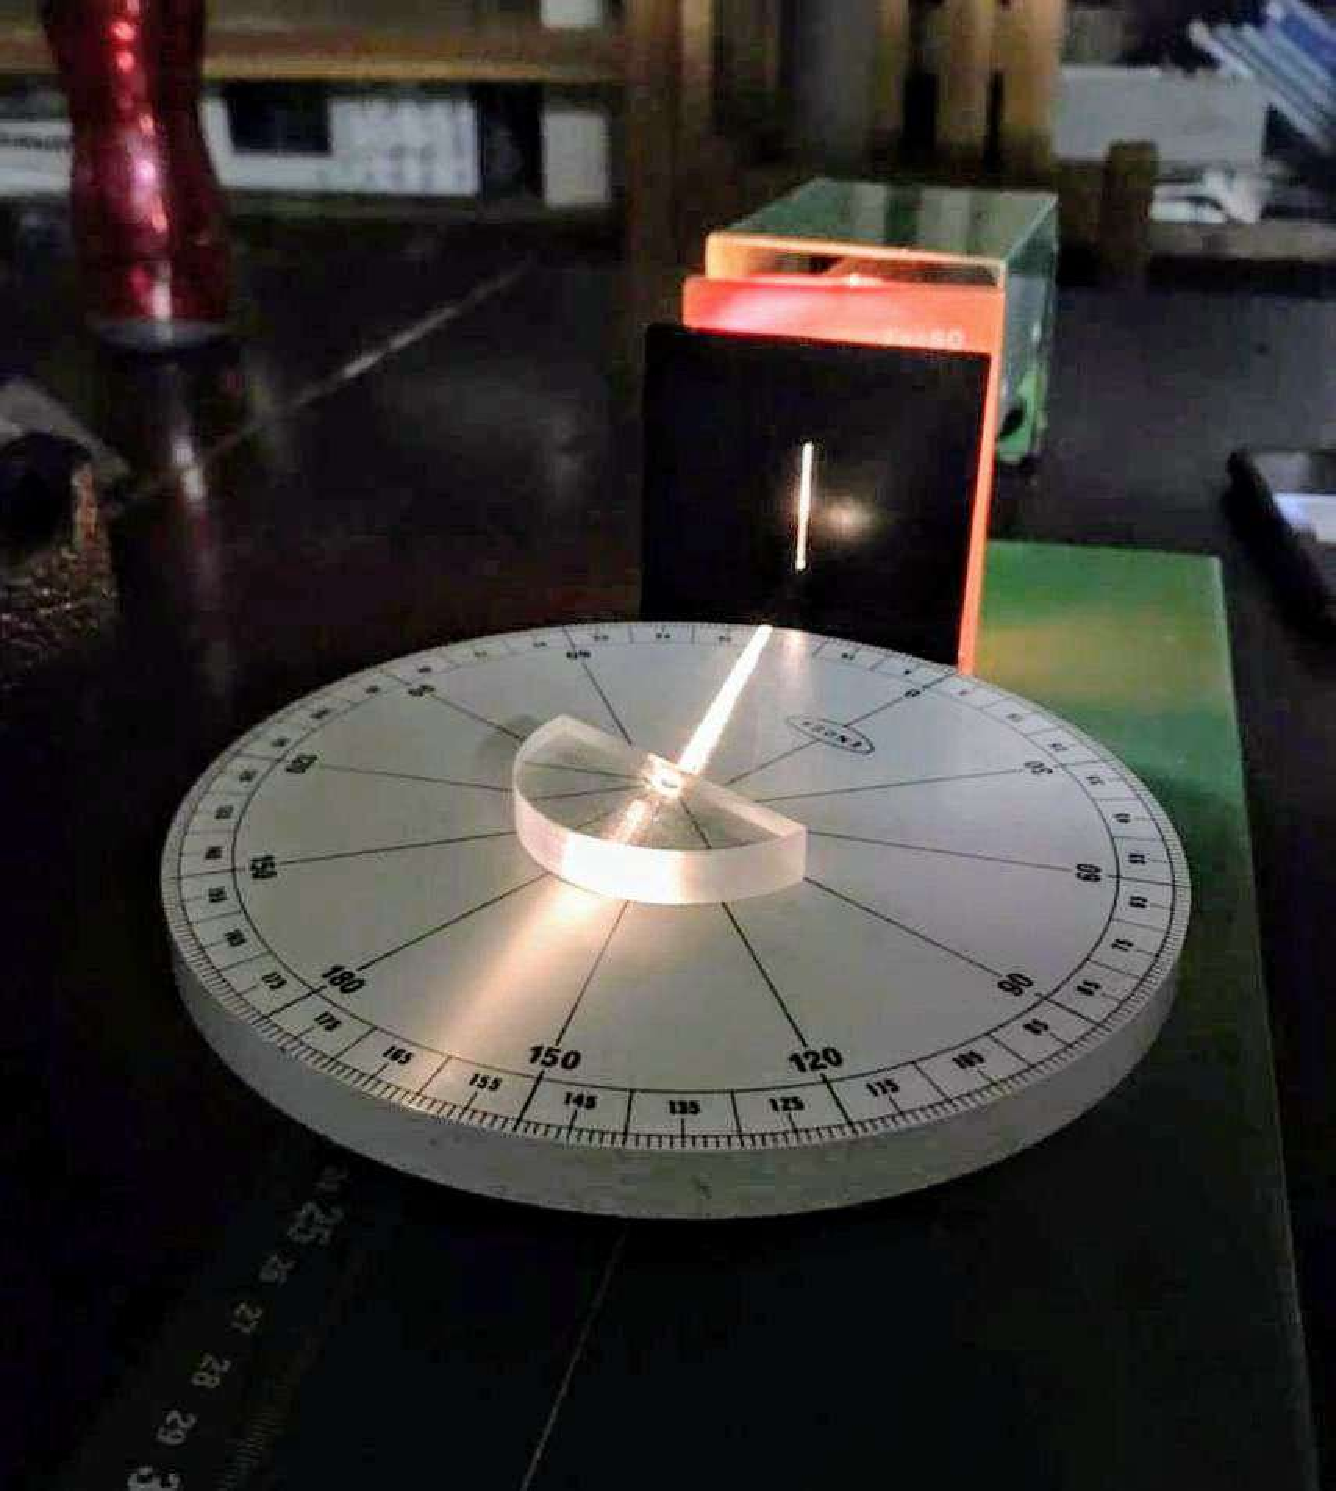
\includegraphics[width=0.5\columnwidth]{img/img1.pdf}
\caption{\label{fig:img_1} Montaje experimental: Refracción de la luz.}
\end{figure}

\section{\label{sec:resultados}Resultados}
\begin{table}[H]%[H] add [H] placement to break table across pages
    \caption{\label{tab:tabla1} Refracción y reflexión de un haz de luz que incide sobre la cara plana de un cilindro semicircular lleno de \textbf{agua}.}
     \begin{ruledtabular}
     \begin{tabular}{ccc}
        Incidente $(\theta_i)$ & Reflejado $(\theta_r)$ & Transmitido $(\theta_t)$\\
        \hline
         0$^{\circ}$ &  0$^{\circ}$ & 0 $^{\circ}$ \\
        10$^{\circ}$ & 10$^{\circ}$ & 7 $^{\circ}$ \\
        20$^{\circ}$ & 19$^{\circ}$ & 14$^{\circ}$ \\
        30$^{\circ}$ & 29$^{\circ}$ & 21$^{\circ}$ \\
        40$^{\circ}$ & 40$^{\circ}$ & 28$^{\circ}$ \\
        50$^{\circ}$ & 50$^{\circ}$ & 34$^{\circ}$ \\
        60$^{\circ}$ & 59$^{\circ}$ & 40$^{\circ}$ \\
        70$^{\circ}$ & 70$^{\circ}$ & 44$^{\circ}$ \\
        80$^{\circ}$ & 81$^{\circ}$ & 48$^{\circ}$ \\
     \end{tabular}
     \end{ruledtabular}
\end{table}

\begin{table}[H]%[H] add [H] placement to break table across pages
    \caption{\label{tab:tabla2} Refracción y reflexión de un haz de luz que incide sobre la cara curvada de un cilindro semicircular lleno de \textbf{agua}. (El agua será considerado como el medio de propagación inicial). En $\theta_i = 49^{\circ}$, el haz transmitido desaparece.}
     \begin{ruledtabular}
     \begin{tabular}{ccc}
        Incidente $(\theta_i)$ & Reflejado $(\theta_r)$ & Transmitido $(\theta_t)$\\
        \hline
         0$^{\circ}$ &  0$^{\circ}$ & 0$^{\circ}$ \\
        10$^{\circ}$ &  9$^{\circ}$ & 14$^{\circ}$ \\
        20$^{\circ}$ & 19$^{\circ}$ & 27$^{\circ}$ \\
        30$^{\circ}$ & 29$^{\circ}$ & 41$^{\circ}$ \\
        40$^{\circ}$ & 39$^{\circ}$ & 59$^{\circ}$ \\
        45$^{\circ}$ & 44$^{\circ}$ & 71$^{\circ}$ \\
        49$^{\circ}$ & 48$^{\circ}$ & --- \\
     \end{tabular}
     \end{ruledtabular}
\end{table}

\begin{table}[H]%[H] add [H] placement to break table across pages
    \caption{\label{tab:tabla 5} Refracción y reflexión de un haz de luz que incide sobre la cara curvada de un cilindro semicircular de algún tipo de \textbf{vidrio}. En $\theta_i = 44^{\circ}$, el haz transmitido desaparece.}
     \begin{ruledtabular}
     \begin{tabular}{ccc}
        Incidente $(\theta_i)$ & Reflejado $(\theta_r)$ & Transmitido $(\theta_t)$\\
        \hline
         0$^{\circ}$ &  0$^{\circ}$ & 0 $^{\circ}$ \\
        15$^{\circ}$ & 14$^{\circ}$ & 21$^{\circ}$ \\
        20$^{\circ}$ & 18$^{\circ}$ & 24$^{\circ}$ \\
        30$^{\circ}$ & 27$^{\circ}$ & 42$^{\circ}$ \\
        40$^{\circ}$ & 38$^{\circ}$ & 67$^{\circ}$ \\  44$^{\circ}$ & 41$^{\circ}$ & --- 
     \end{tabular}
     \end{ruledtabular}
\end{table}


\begin{figure}
\centering
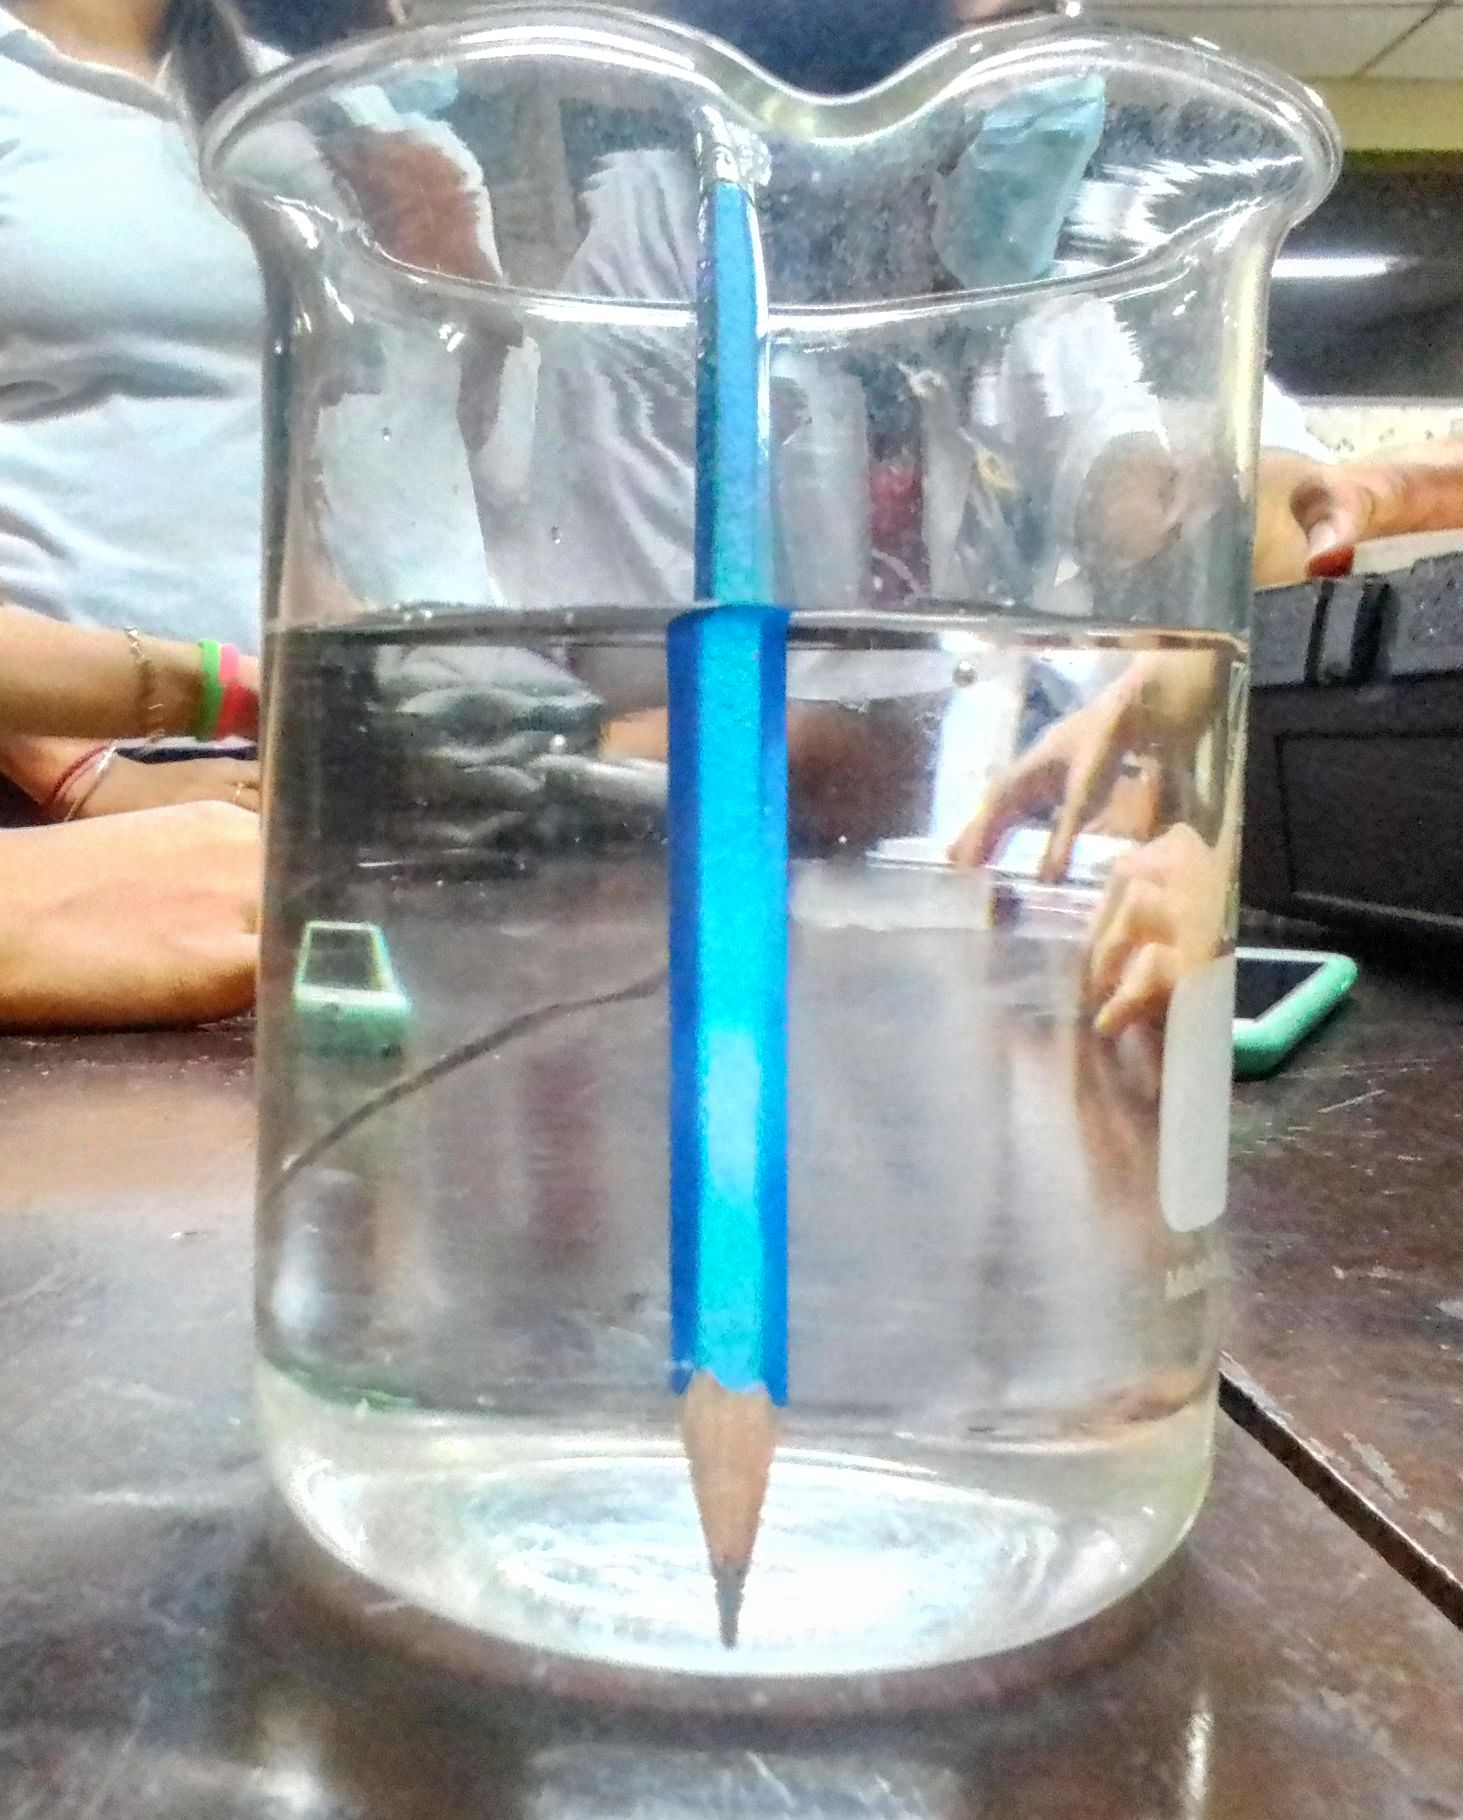
\includegraphics[width=0.5\columnwidth]{img/img0.jpg}
\caption{\label{fig:img0}Refracción de luz: cara frontal}
\end{figure}

\begin{figure}
\centering
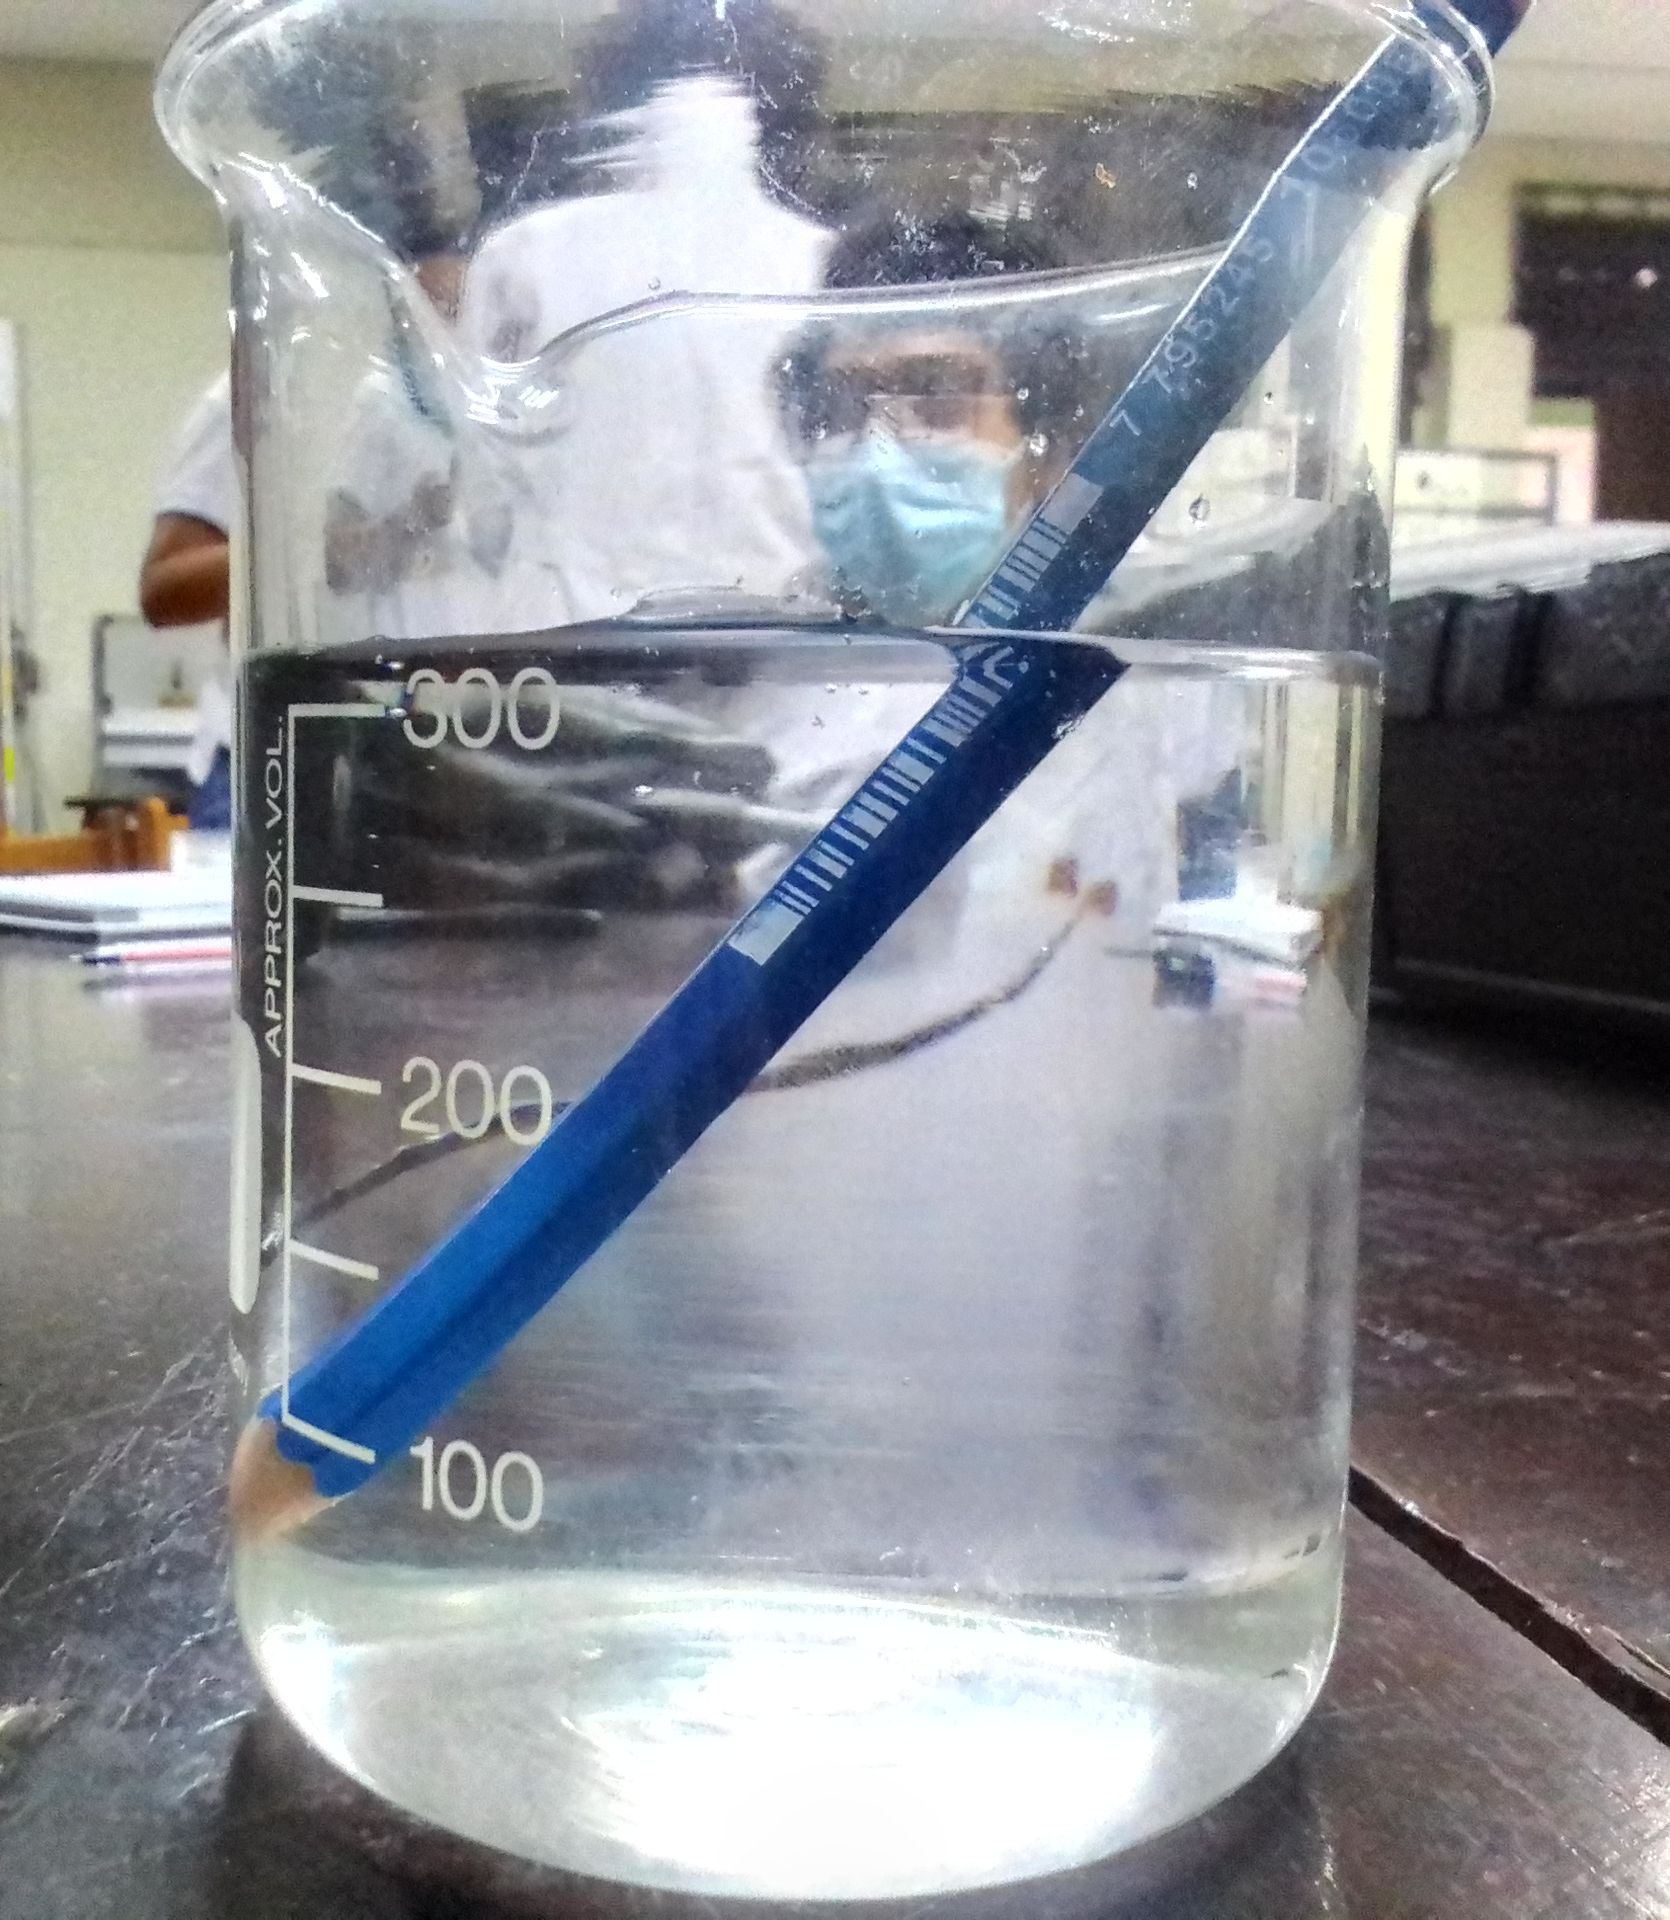
\includegraphics[width=0.5\columnwidth]{img/img1.jpg}
\caption{\label{fig:img1}Refracción de luz: cara lateral}
\end{figure}
\begin{figure}
\centering
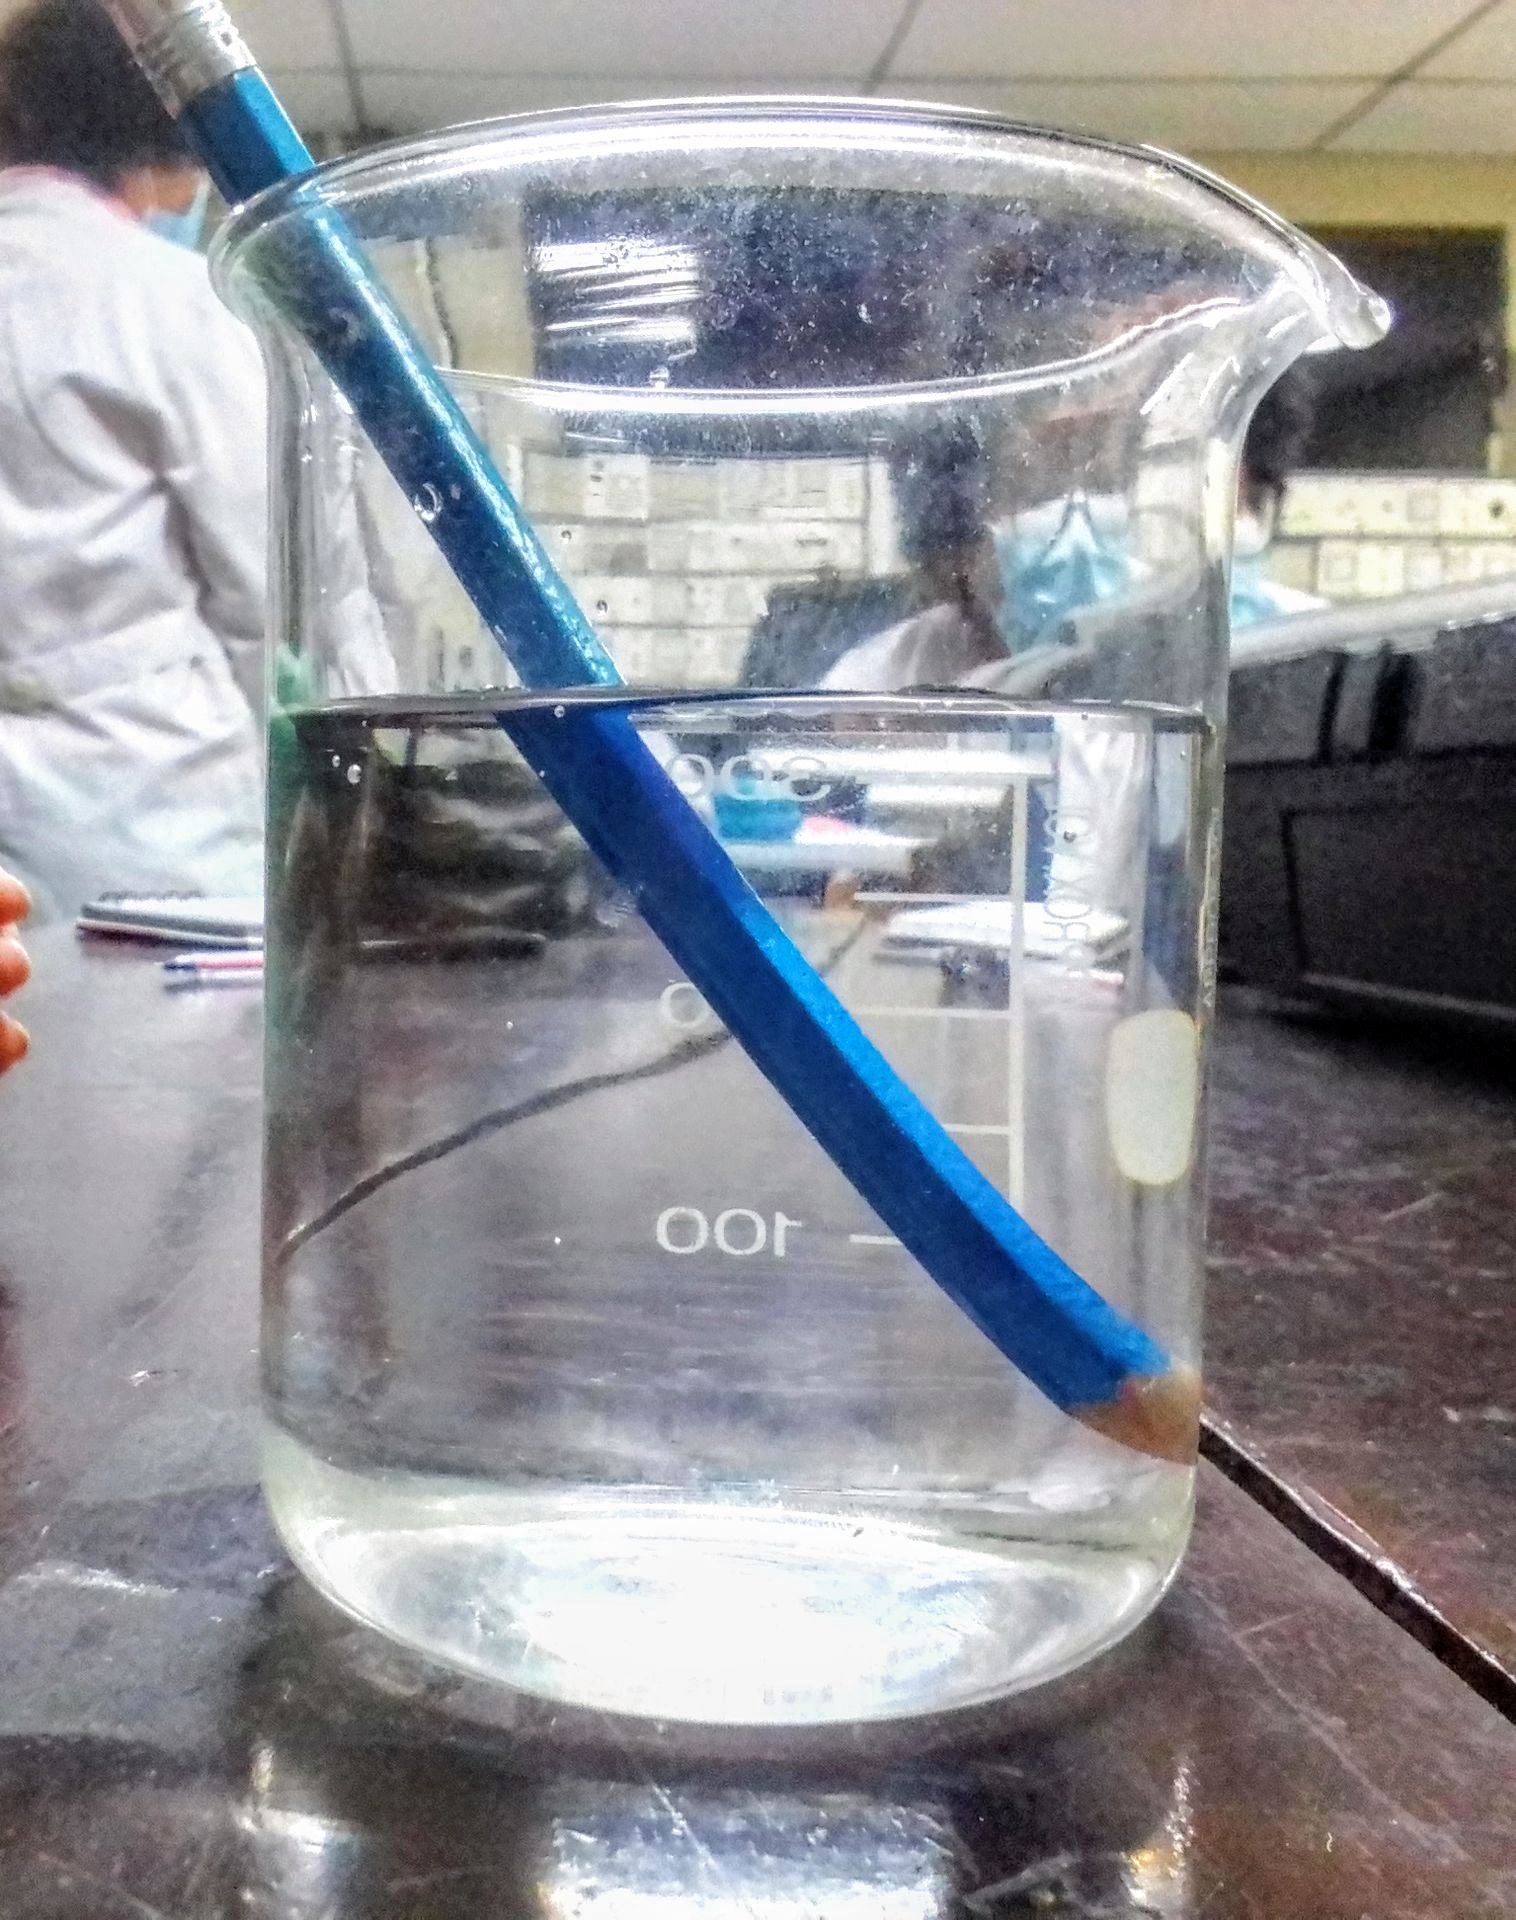
\includegraphics[width=0.5\columnwidth]{img/img2.jpg}
\caption{\label{fig:img2}Refracción de luz: cara lateral}
\end{figure}
\begin{figure}
\centering
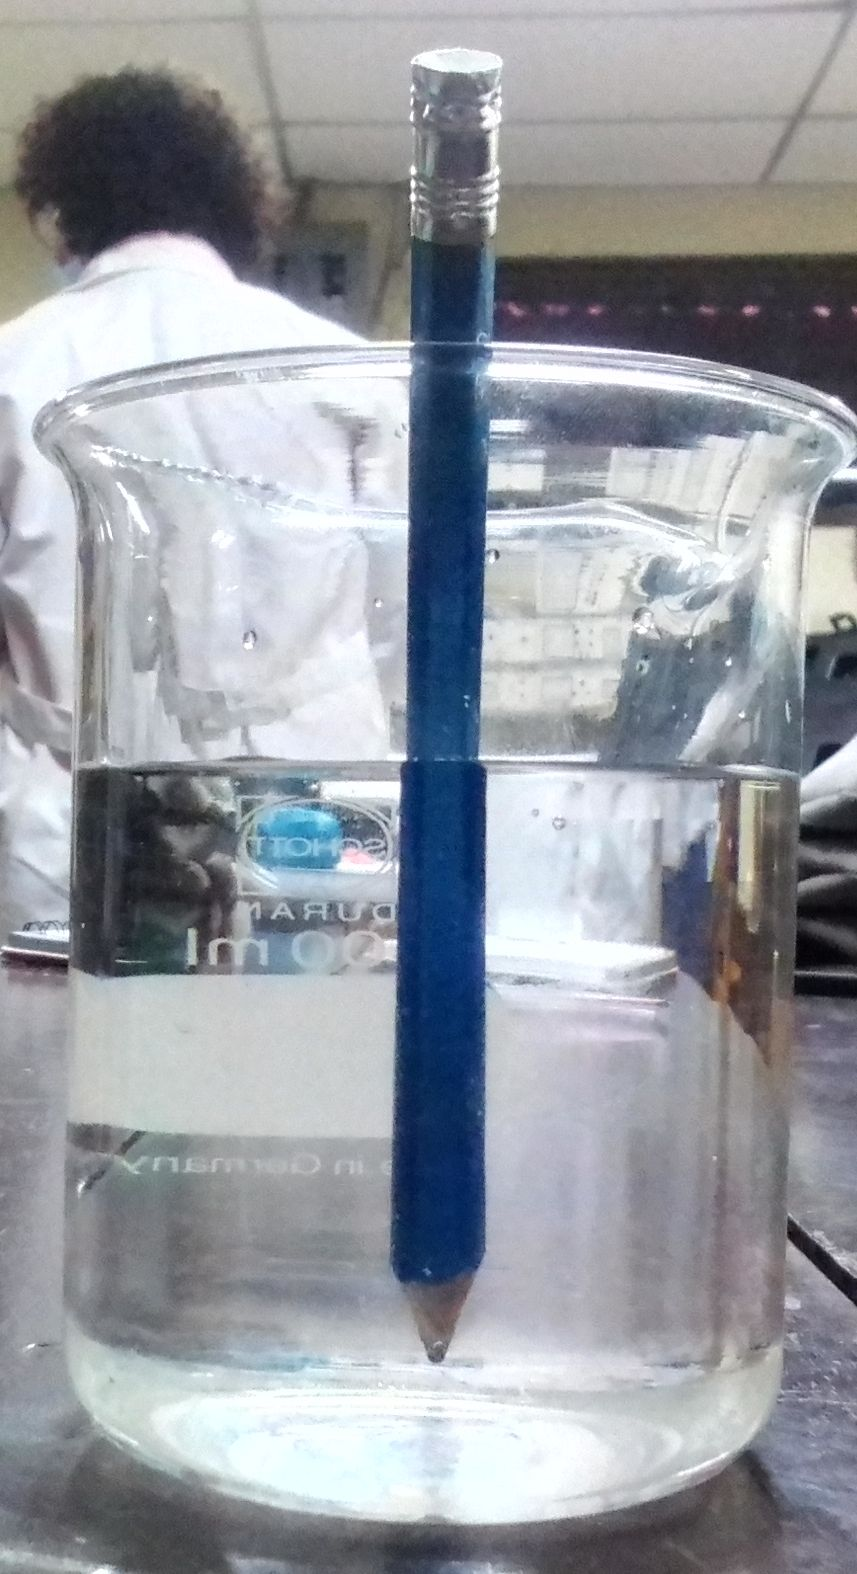
\includegraphics[width=0.45\columnwidth]{img/img3.jpg}
\caption{\label{fig:img3}Refracción de luz: cara trasera}
\end{figure}


\section{Análisis}

Mediante la ley de Snell, resulta pertinente encontrar el índice de refracción del agua mediante los datos de la tabla \ref{tab:tabla1} y \ref{tab:tabla2}. (Observe las gráficas de las figuras \ref{fig:grafica0} y \ref{fig:grafica1})

\begin{figure}
\centering
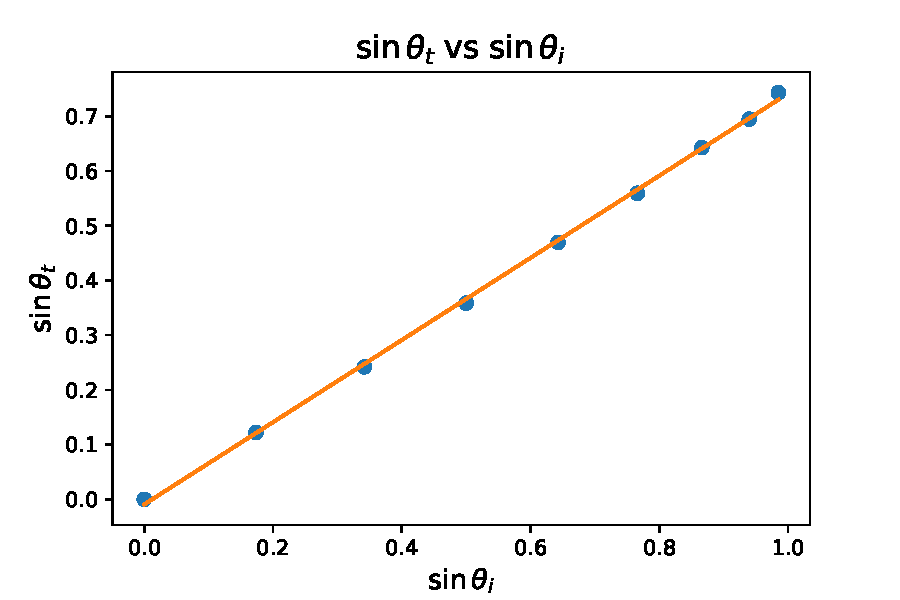
\includegraphics[width=\columnwidth]{img/grafica0.pdf}
\caption{\label{fig:grafica0}Relación entre el seno del ángulo de incidencia con respecto al transmitido cuando el haz de luz incide sobre la cara \textbf{plana} de un cilindro con agua.}
\end{figure}

\begin{figure}
\centering
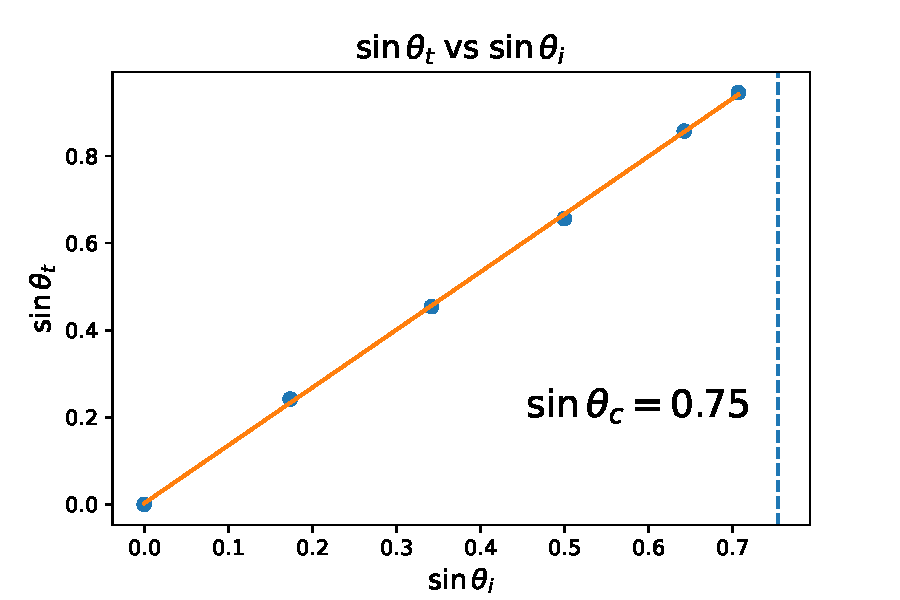
\includegraphics[width=\columnwidth]{img/grafica1.pdf}
\caption{\label{fig:grafica1}Relación entre el seno del ángulo de incidencia con respecto al transmitido cuando el haz de luz incide sobre la cara \textbf{curva} de un cilindro con agua. Cuando $\theta_i=\theta_c=49$, no existe un valor correspondiente para $\theta_t$.}
\end{figure}

De las cuales se extrae que el índice de refracción del agua (en ambos casos) es $n_{\text{agua}}= 1.332$. Compararando este valor con el reportado en la tabla \ref{tab:indices}, el error porcentual del índice de refracción del agua es $E_r=0.07\%$.

\subsection{Medios con distinto Índice de Refracción}

La teoría afirma que el fenómeno de la Refracción se produce en la superficie de separación de dos medios; cada uno con diferentes características, entre estas la densidad del medio. En la refracción de la luz se distingue el rayo incidente y el rayo refractado y sus formaciones angulares respecto a la línea normal. De acuerdo con los resultados mostrados en las tablas \ref{tab:tabla2} y \ref{tab:tabla 5}, se puede pueden observar variaciones en el ángulo de refracción para cuando el primer medio tiene mayor índice de refracción que el segundo, y tambien se puede notar que solamente bajo estas condiciones, el haz de luz transmitido desaparece para cierto ángulo de incidencia.

\begin{table}[H]
	\caption{\label{tab:indices} Algunos Materiales y sus índices de Refracción}
	\begin{ruledtabular}
		\begin{tabular}{lcc}
            \textrm{Materiales} & \textrm{} & \textrm{Índice $(n)$}\\
			\colrule
			Diamante            & --------- & 2,4200\\
            Ámbar               & --------- & 1,5400\\
            Agua                & --------- & 1,3300\\
            Vidrio (común)      & --------- & 1,4500\\
            Plástico            & --------- & 1,4900\\
            Aire                & --------- & 1,0000\\
	\end{tabular}
	\end{ruledtabular}
\end{table}

En la tabla anterior, se muestran algunos índices de refracción de algunos materiales; entre ellos, $\textit{el vidrio}$ y $\textit{el agua}$. Ahora, se analiza lo que ocurre para los casos:
\begin{align*}
    n_{t} > n_{i}\\
    n_{i} > n_{t}
\end{align*}
Considerando que para esta práctica, los índices de refracción utilizados como primer medio de incidencia fueron: el vidrio $= 1.45$ y el agua $= 1.33$. Estos poseen un mayor índice de refracción que el segundo medio (en ambos casos) el aire $1.00$. De este modo se cumple que $n_{i} > n_{t}$. \\

De acuerdo con la tabla \ref{tab:tabla2}, se observa que los ángulos con que el rayo de luz incide $(\theta_i)$ en este medio (agua), son menores a los ángulos con que se refracta ($\theta_t$) en el segundo medio (aire). Esto demuestra la relación que existe entre el ángulo de incidencia y el refractado, para cuando el primer medio, tiene mayor índice de refracción.
\begin{align*}
\text{Si},\;\; n_{i} > n_{t} \Longrightarrow \theta_{t} > \theta_{i}    
\end{align*}
Esto sucede debido a que la velocidad de la luz, depende del medio; por lo que es más lenta cuanto más denso sea el material. Por ello, si el rayo de luz pasa de un medio más denso a uno menos denso, será refractado \textbf{alejándose de la normal} y, por tanto, el ángulo de incidencia será menor que el de refracción. \\
\\
El índice de refracción determina cuánto se desvía o se refracta la trayectoria de la luz al entrar en un material. Esto se describe mediante la ley de refracción de Snell, (\ref{eqn:ley_snell}) descrita en la teoría.\\
\\
En las tablas también se observa, que para cierto ángulo de incidencia; el rayo refractado desaparece. En el caso de la tabla \ref{tab:tabla 5}, cuando el rayo incide con un ángulo de $44^{\circ}$, no se produce ángulo transmitido. Este fenómeno se denomina, \textbf{Reflexión total interna} y se produce solo para las refracciones estudiadas $(n_{i} > n_{t})$ cuando el rayo incide con un ángulo tal que no es capaz de atravesar la superficie entre ambos medios. A este ángulo, se le denomina \textbf{Ángulo critico} y es derivado de la \textit{Ley de Snell}.

\begin{align*}
    \theta_{c} = sen^{-1}\left(\frac{n_{2}}{n_{1}}\right)
\end{align*}

\begin{figure}[H]
\centering
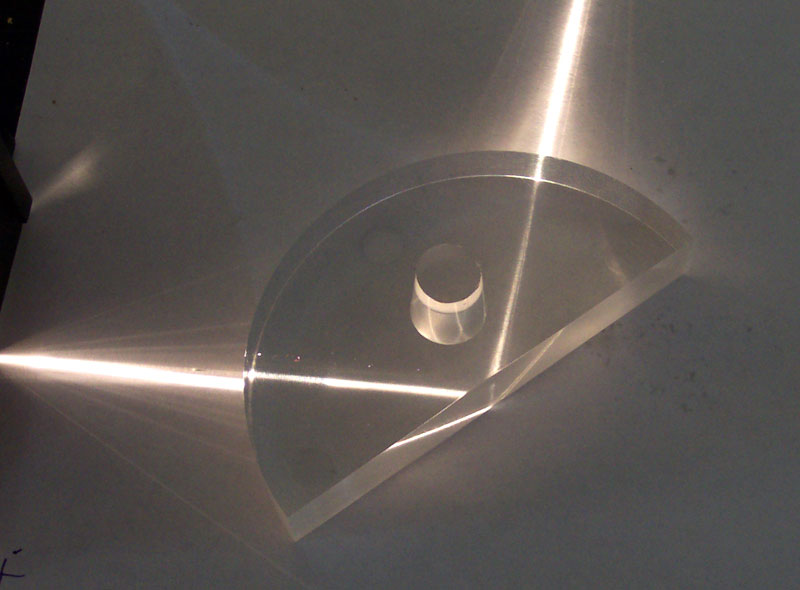
\includegraphics[width=0.5\columnwidth]{img/Total_internal_reflection.jpg}
\caption{\label{fig:g1} Reflexión Total Interna}
\end{figure}

El principio de la refracción, se puede estudiar también en el sistema del lápiz que se introduce en un vaso de precipitado (observe las figuras \ref{fig:img0}, \ref{fig:img1}, \ref{fig:img2} y \ref{fig:img3}).\\
\\
La imagen muestra una aparente \textbf{ruptura} en el lápiz, al entrar en contacto con le agua. De los resultados analizados en las imágenes d, se puede deducir que cuanto más elevado es el índice de refracción, mayor es la reducción de velocidad que sufre la luz en ese medio y mas se afecta la dirección de esta con respecto a la normal. Por lo tanto, en el experimento del lápiz, ocurre que la luz viaja en linea recta desde la parte sumergida, hasta el observador, pero una vez atraviesa la interfase y entra en contacto con el segundo medio (aire), esta se desvía creando una sensación de dispersión en la forma original del objeto visto por el observador.

\section{Conclusiones}

De acuerdo a lo expuesto, se concluyó que bajo la condición de que el índice de refracción de los medios $n_i  > n_t$ (índice de refracción del medio de incidencia es mayor que el índice del medio de refracción), para cierto ángulo límite o ángulo crítico, el haz de luz refractado desaparece y por ende, toda la luz es reflejeda. La razón de este fenómeno se asocia a que la alta densidad de los medios reduce la velocidad de propagación del haz de luz.

Cabe resaltar que para que este fenómeno se cumpla; la luz debe incidir de forma oblicua sobre la superficie de separación entre los medios y para el caso en que pasa de un medio $(n_{i}>n_{t})$, se va a producir la reflexión total interna, que aplica para un ángulo limite en el cual el rayo de luz debido a su inclinación y bajo características del medio, no puede atravesar la linea interfase.



\bibliography{report_physics}
\end{document}